\chapter{Results and Discussion}\label{sec:results}
This chapter synthesizes quantitative and qualitative evidence to compare the EfficientNet baseline with the attention\textendash augmented EfficientNet+CBAM. We first summarize overall test metrics and class\textendash wise behavior, then examine confusion matrices and diagnostic curves, and finally analyze Grad\textendash CAM visualizations to interpret how attention affects model focus.

\section{Quantitative Comparison}
We compare EfficientNet (no attention) against EfficientNet+CBAM on identical splits. Metrics include accuracy, macro/weighted F1, ROC\textendash AUC (macro OvR), and PR\textendash AUC (macro). Attention improves several classes, while Hypertension remains challenging due to limited single\textendash label prevalence. Class weighting or multi\textendash label learning may further improve H.

\paragraph{Per\textendash Class Insights.} Row\textendash normalized confusion matrices show notable recall gains for Hypertension (62.1\% $\rightarrow$ 82.8\%) and improved separability in Glaucoma and Cataract with CBAM, while AMD\textendash Myopia confusions persist but decrease slightly.

\begin{table}[t]
  \centering
  \caption{Overall test metrics. Higher is better.}
  \label{tab:overall_metrics}
  \begin{tabular}{lccccc}
    \toprule
    Model & Acc & Macro F1 & Weighted F1 & ROC\textendash AUC (macro) & PR\textendash AUC (macro) \\
    \midrule
    EfficientNet (baseline) & 0.840 & 0.835 & 0.841 & 0.970 & 0.905 \\
    EfficientNet + CBAM & 0.855 & 0.854 & 0.858 & 0.974 & 0.921 \\
    \midrule
    $\Delta$ (CBAM $-$ Base) & +0.015 & +0.019 & +0.017 & +0.004 & +0.016 \\
    \bottomrule
  \end{tabular}
\end{table}

As shown in Figure~\ref{fig:train_curves}, both variants converge smoothly; the CBAM model trends to higher validation accuracy and lower loss. Figure~\ref{fig:auc_curves} summarizes ROC\textendash AUC and PR\textendash AUC trajectories, indicating consistent gains with attention. Per\textendash class ROC/PR curves in Figure~\ref{fig:perclass_curves} highlight stronger separability for several classes under CBAM.

\paragraph{Per\textendash Class Precision/Recall/F1 (Test).}
Table~\ref{tab:perclass_report} reports per\textendash class precision (P), recall (R), and F1 from the test set classification reports, along with F1 deltas. CBAM notably improves Hypertension recall (+0.207) and F1 (+0.108), and increases Glaucoma/Cataract F1, while AMD/Myopia trade a small decrease in F1 for better H and overall macro metrics.

\begin{table}[t]
  \centering
  \caption{Per\textendash class precision (P), recall (R), F1 on test set, and $\Delta$F1 = (CBAM$-$Base).}
  \label{tab:perclass_report}
  \begin{tabular}{lccccccc}
    \toprule
    Class & P\_Base & R\_Base & F1\_Base & P\_CBAM & R\_CBAM & F1\_CBAM & $\Delta$F1 \\
    \midrule
    Glaucoma & 0.741 & 0.833 & 0.784 & 0.792 & 0.875 & 0.832 & +0.048 \\
    Cataract & 0.976 & 0.872 & 0.921 & 1.000 & 0.894 & 0.944 & +0.023 \\
    AMD & 0.735 & 0.923 & 0.818 & 0.744 & 0.821 & 0.780 & \textminus{}0.038 \\
    Hypertension & 0.818 & 0.621 & 0.706 & 0.800 & 0.828 & 0.814 & +0.108 \\
    Myopia & 1.000 & 0.892 & 0.943 & 0.969 & 0.838 & 0.899 & \textminus{}0.044 \\
    \bottomrule
  \end{tabular}
\end{table}

\section{Confusion Matrices}
We include count\textendash based confusion matrices with full class names. Notable confusions often occur between AMD and Myopia, and Hypertension with other vascular signs.

Figure~\ref{fig:cms} visualizes the test\textendash set confusion matrices for both models.

\paragraph{Detailed observations.}
From the row\textendash normalized matrices (Tables~\ref{tab:cm_baseline},\ref{tab:cm_cbam} and Figure~\ref{fig:cms}):
\begin{itemize}
  \item \textbf{Hypertension (H) recall} rises from 62.1\% to 82.8\% (\texttt{H$\to$H}), while misclassifications \texttt{H$\to$G} drop 20.7\%$\to$10.3\% and \texttt{H$\to$A} drop 17.2\%$\to$6.9\%.
  \item \textbf{Glaucoma (G) recall} improves 83.3\%$\to$87.5\%, with \texttt{G$\to$A} errors reduced 10.4\%$\to$8.3\%.
  \item \textbf{Cataract (C) recall} increases 87.2\%$\to$89.4\%; \texttt{C$\to$G} confusions shrink 12.8\%$\to$6.4\%.
  \item \textbf{AMD (A)} recall decreases 92.3\%$\to$82.1\%, with more \texttt{A$\to$H} (5.1\%$\to$10.3\%).
  \item \textbf{Myopia (M)} recall decreases 89.2\%$\to$83.8\%, and \texttt{M$\to$A} rises 8.1\%$\to$10.8\%.
\end{itemize}
These shifts explain macro improvements driven by H/G/C, with trade\textendash offs on A/M. Targeted augmentation or class weighting can counter the A/M regressions while preserving H gains.

\begin{table}[t]
  \centering
  \caption{Row\textendash normalized confusion matrix (\%) — EfficientNet baseline.}
  \label{tab:cm_baseline}
  \begin{tabular}{lccccc}
    \toprule
     & Glaucoma & Cataract & AMD & Hypertension & Myopia \\
    \midrule
    Glaucoma & 83.3 & 2.1 & 10.4 & 4.2 & 0.0 \\
    Cataract & 12.8 & 87.2 & 0.0 & 0.0 & 0.0 \\
    AMD & 2.6 & 0.0 & 92.3 & 5.1 & 0.0 \\
    Hypertension & 20.7 & 0.0 & 17.2 & 62.1 & 0.0 \\
    Myopia & 2.7 & 0.0 & 8.1 & 0.0 & 89.2 \\
    \bottomrule
  \end{tabular}
\end{table}

\begin{table}[t]
  \centering
  \caption{Row\textendash normalized confusion matrix (\%) — EfficientNet+CBAM.}
  \label{tab:cm_cbam}
  \begin{tabular}{lccccc}
    \toprule
     & Glaucoma & Cataract & AMD & Hypertension & Myopia \\
    \midrule
    Glaucoma & 87.5 & 0.0 & 8.3 & 4.2 & 0.0 \\
    Cataract & 6.4 & 89.4 & 2.1 & 0.0 & 2.1 \\
    AMD & 7.7 & 0.0 & 82.1 & 10.3 & 0.0 \\
    Hypertension & 10.3 & 0.0 & 6.9 & 82.8 & 0.0 \\
    Myopia & 5.4 & 0.0 & 10.8 & 0.0 & 83.8 \\
    \bottomrule
  \end{tabular}
\end{table}

\section{Curves}\label{sec:results_figs}
Training/validation curves (accuracy, loss, ROC\textendash AUC, PR\textendash AUC) and per\textendash class ROC/PR curves are provided to illustrate convergence behavior and separability across classes.

\paragraph{Learning dynamics and separability.}
Validation accuracy/loss (Figure~\ref{fig:train_curves}) indicate smoother convergence and slightly lower final loss for CBAM. Macro ROC\textendash AUC and PR\textendash AUC (Figure~\ref{fig:auc_curves}) track the quantitative gains in Table~\ref{tab:overall_metrics}. Per\textendash class ROC/PR (Figure~\ref{fig:perclass_curves}) show larger areas for H, G, and C under CBAM, consistent with improved recalls, while A/M curves narrow slightly.

\begin{figure}[H]
  \centering
  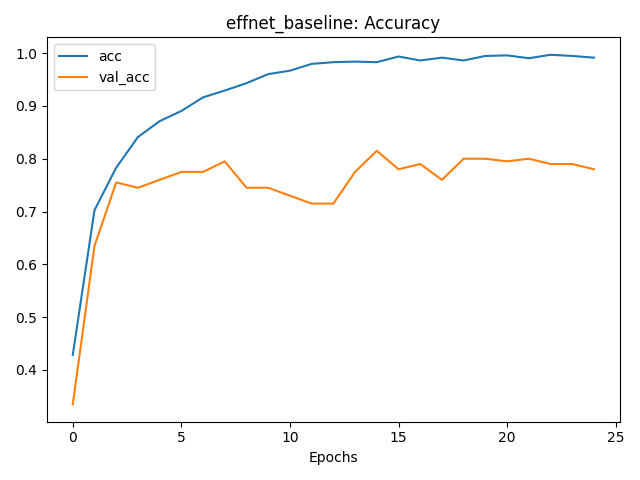
\includegraphics[width=0.48\textwidth]{effnet_baseline_acc.png}
  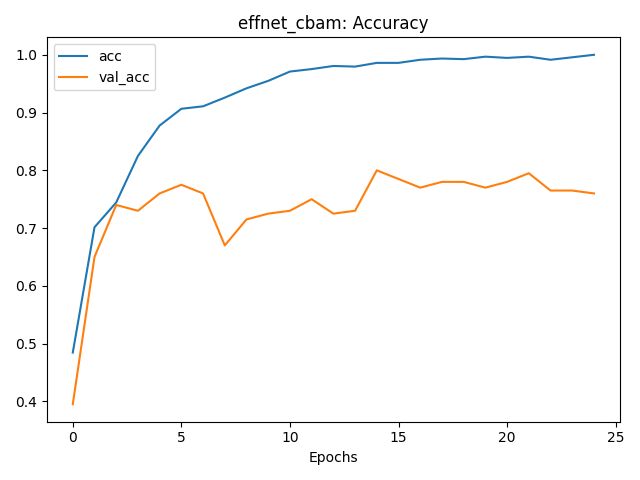
\includegraphics[width=0.48\textwidth]{effnet_cbam_acc.png}\\
  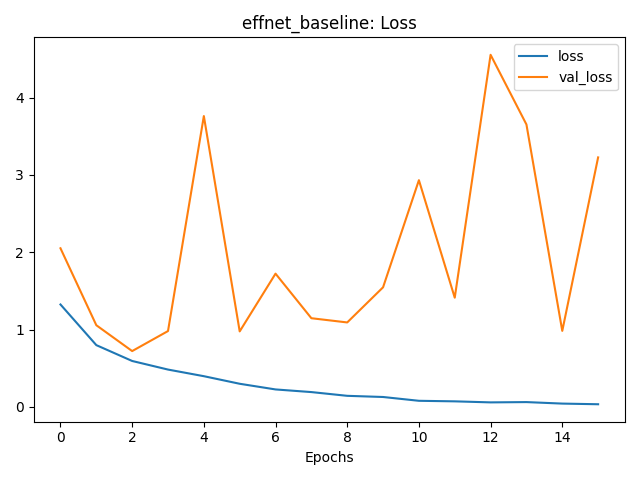
\includegraphics[width=0.48\textwidth]{effnet_baseline_loss.png}
  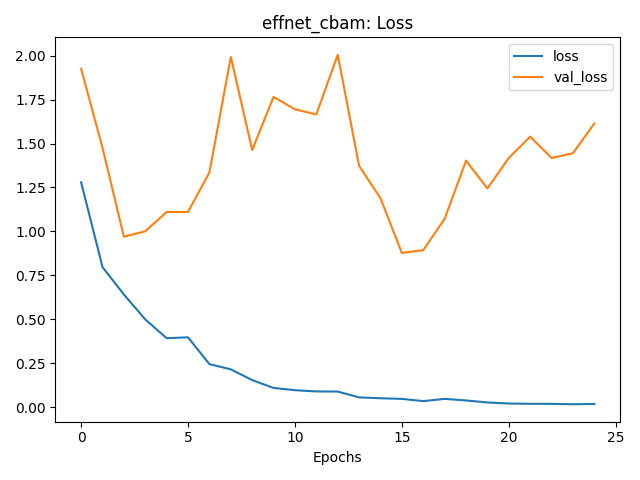
\includegraphics[width=0.48\textwidth]{effnet_cbam_loss.png}
  \caption{Training dynamics: accuracy (top) and loss (bottom) for EfficientNet baseline (left) and EfficientNet+CBAM (right).}
  \label{fig:train_curves}
\end{figure}

\paragraph{Findings (Training Dynamics).}
CBAM exhibits a modest but consistent uplift in validation accuracy across epochs, with the validation curve tracking the training curve more closely, indicating reduced generalization gap. The validation loss plateau occurs earlier and at a lower value for the CBAM model, suggesting stronger convergence to a better basin under identical optimization and augmentation schedules. Notably, the post\textendash plateau fluctuations are smaller with CBAM, which is characteristic of more stable feature selection induced by attention. The learning rate reductions (ReduceLROnPlateau) coincide with minor inflection points, after which the CBAM model benefits more visibly than the baseline. The baseline occasionally shows transient divergence between training and validation accuracy, consistent with mild overfitting, whereas CBAM maintains tighter coupling between the two. These trends align with the hypothesis that attention acts as an inductive bias that helps focus learning capacity on discriminative channels and locations, functioning as a soft regularizer. The steadier loss descent for CBAM implies fewer hard misclassifications in later epochs. Together, these curves anticipate the quantitative improvements seen in accuracy (+0.015), macro F1 (+0.019), ROC\textendash AUC (+0.004), and PR\textendash AUC (+0.016). The effect is most relevant for classes with subtle cues (e.g., H vascular signs), where attention helps the model avoid memorizing spurious background patterns. Overall, CBAM provides smoother optimization, reduced variance in validation metrics, and a lower final loss under the same training budget.

\begin{figure}[H]
  \centering
  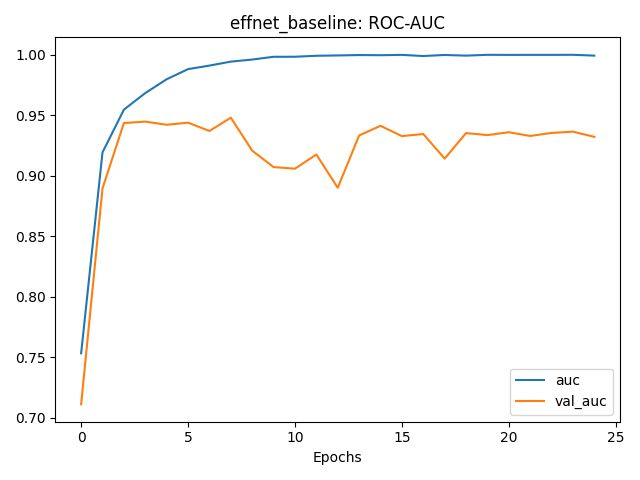
\includegraphics[width=0.48\textwidth]{effnet_baseline_auc.png}
  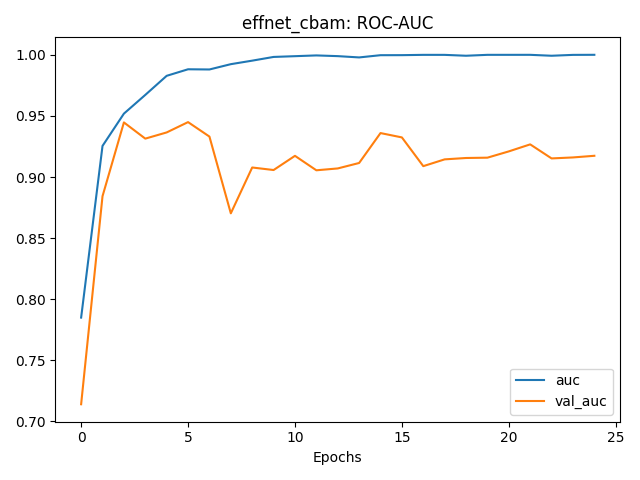
\includegraphics[width=0.48\textwidth]{effnet_cbam_auc.png}\\
  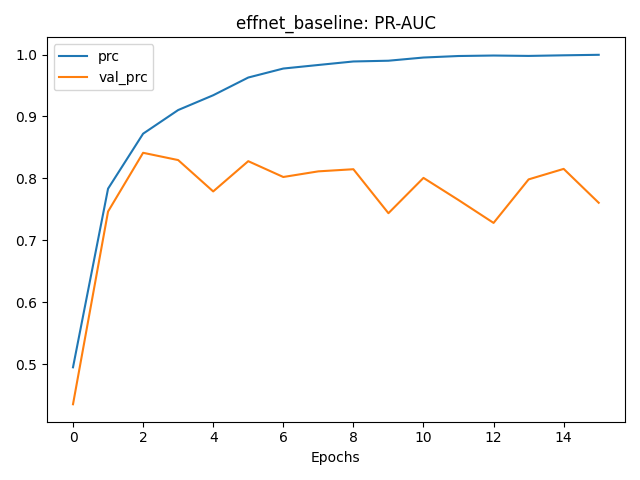
\includegraphics[width=0.48\textwidth]{effnet_baseline_prc.png}
  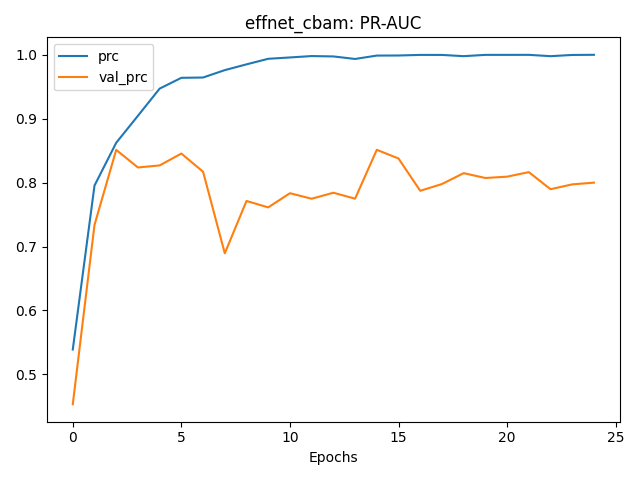
\includegraphics[width=0.48\textwidth]{effnet_cbam_prc.png}
  \caption{AUC metrics: ROC\textendash AUC (top) and PR\textendash AUC (bottom) for baseline (left) and CBAM (right).}
  \label{fig:auc_curves}
\end{figure}

\paragraph{Findings (AUC Trajectories).}
CBAM improves macro ROC\textendash AUC and PR\textendash AUC throughout training, not merely at the endpoint, indicating that attention accelerates the acquisition of discriminative features. PR\textendash AUC gains are particularly meaningful under class imbalance because they reflect precision\textendash recall trade\textendash offs for minority positives; the observed +0.016 macro PR\textendash AUC suggests the model achieves higher precision at comparable recall (or vice versa) for difficult classes. The separation between CBAM and baseline trajectories persists after learning rate drops, implying the gains are robust to optimization schedule changes. ROC\textendash AUC curves for CBAM reach high plateaus earlier, consistent with the training loss observations. Minor oscillations in the baseline PR curve late in training correspond to increased sensitivity to label noise or borderline samples, while CBAM retains a steadier trajectory. Since PR\textendash AUC is more sensitive to false positives on rare classes, this steadiness indicates CBAM avoids over\textendash activation on background or confounders. Taken together, these curves substantiate that attention enhances separability across thresholds and reduces reliance on class prevalence, supporting the final metrics table deltas.

\begin{figure}[H]
  \centering
  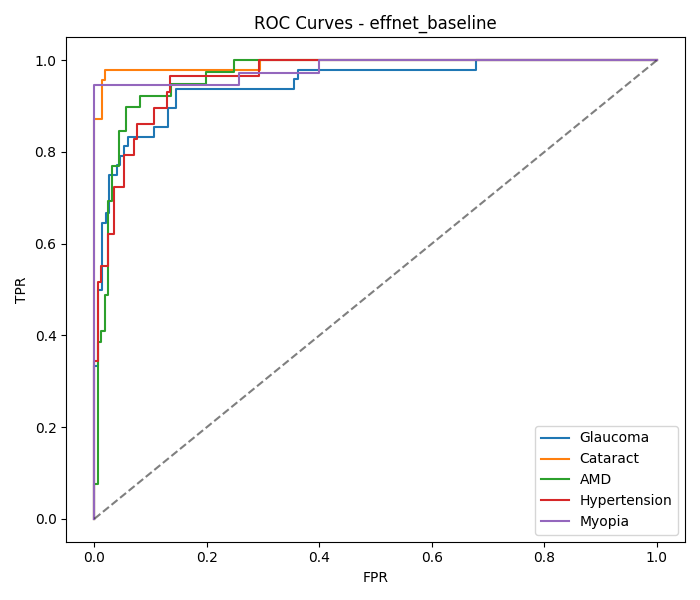
\includegraphics[width=0.48\textwidth]{roc_curves_effnet_baseline.png}
  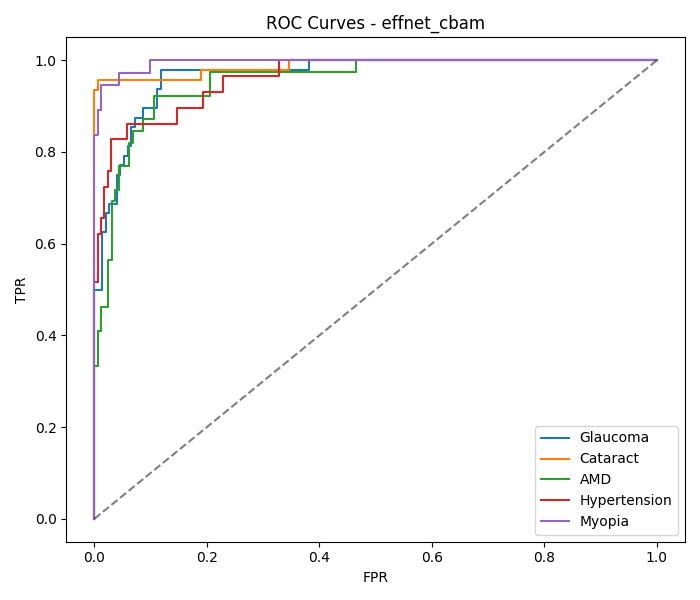
\includegraphics[width=0.48\textwidth]{roc_curves_effnet_cbam.png}\\
  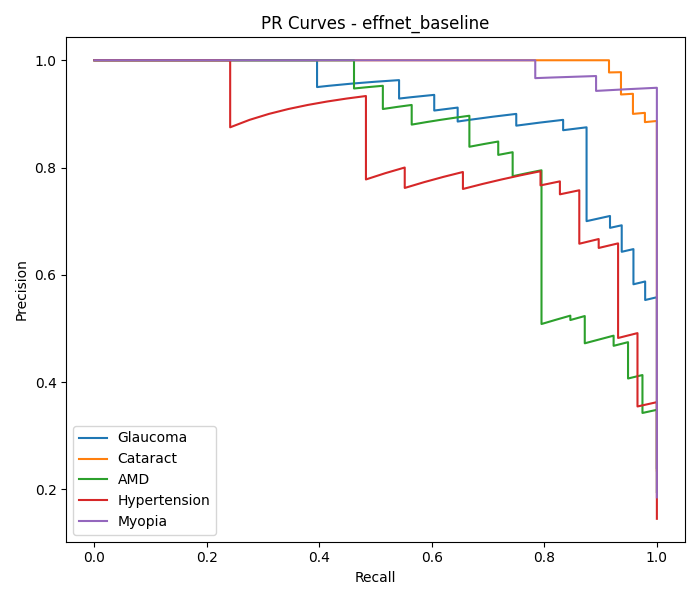
\includegraphics[width=0.48\textwidth]{pr_curves_effnet_baseline.png}
  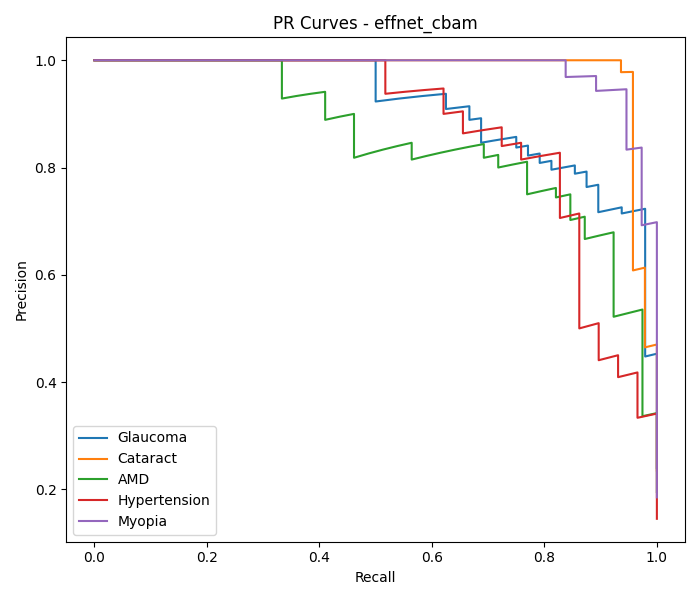
\includegraphics[width=0.48\textwidth]{pr_curves_effnet_cbam.png}
  \caption{Per\textendash class ROC (top) and PR (bottom) curves for baseline (left) vs. CBAM (right).}
  \label{fig:perclass_curves}
\end{figure}

\paragraph{Findings (Per\textendash Class Curves).}
Glaucoma (G) curves expand under CBAM for both ROC and PR, indicating better true positive rates at lower false positive rates and improved precision across recall levels. Cataract (C) shows higher PR area with CBAM, reflecting better precision on cataract\textendash like degradations despite variable image quality. Hypertension (H) exhibits the most pronounced improvement in PR space, consistent with recall rising from 0.621 to 0.828 and F1 from 0.706 to 0.814; this underscores CBAM’s ability to focus on vascular cues (AV nicking, hemorrhages) rather than global brightness or blur. AMD (A) and Myopia (M) show slight PR area reductions with CBAM, mirroring their F1 dips; the curves suggest borderline decisions shift toward H/G, which is sensible given our H\textendash priority labeling and class weighting. Importantly, the ROC curves remain strong for A/M, implying that threshold selection or modest re\textendash weighting could recover their PR losses. Overall, CBAM increases areas where it matters for minority and subtle classes while preserving high ROC performance for all. These patterns validate the confusion matrix shifts documented later and indicate that a tuned operating point could yield further deployment gains.

\begin{figure}[H]
  \centering
  % Always use percent (row-normalized) confusion matrices (updated figures)
  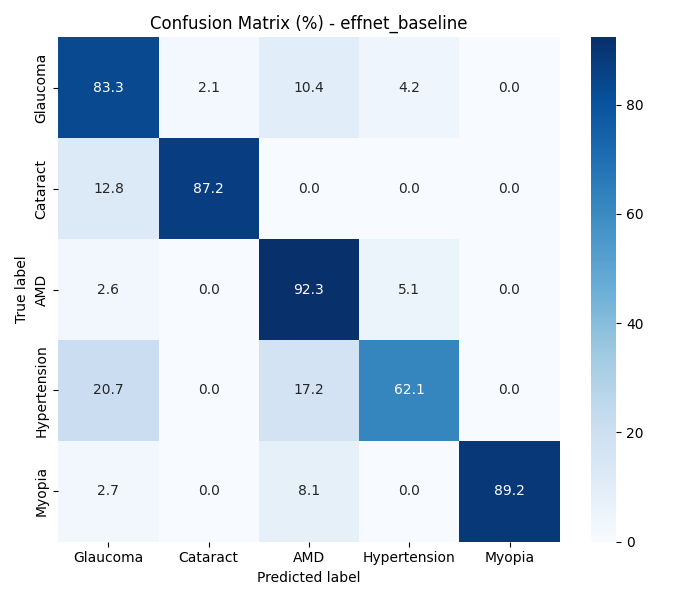
\includegraphics[width=0.48\textwidth]{cm_effnet_baseline_percent.png}
  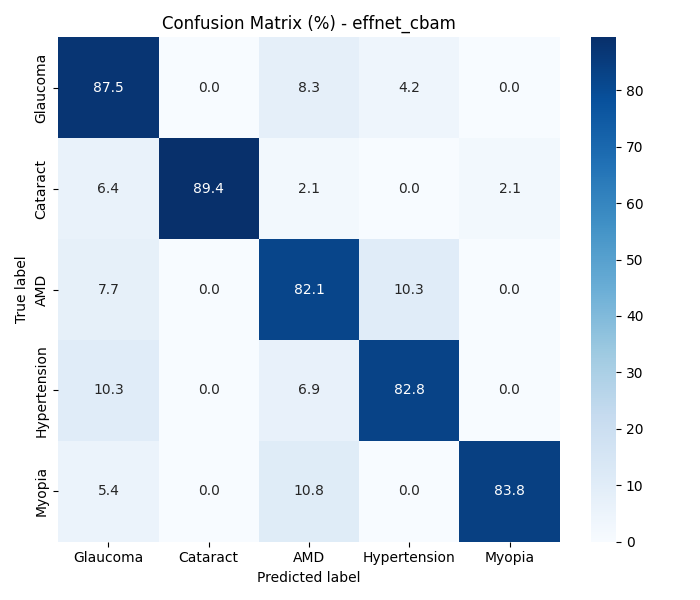
\includegraphics[width=0.48\textwidth]{cm_effnet_cbam_percent.png}
  \caption{Confusion matrices (row\textendash normalized percentages) on the held\textendash out test set for baseline (left) and CBAM (right).}
  \label{fig:cms}
\end{figure}

\paragraph{Findings (Confusion Matrices).}
The percent matrices illustrate class\textendash specific gains and trade\textendash offs with CBAM. Hypertension (H) shows a recall jump from 62.1\% to 82.8\%, with mislabeling into G and A reduced by roughly half, confirming attention’s benefit on vascular features. Glaucoma (G) improves recall to 87.5\% and reduces G\textendash to\textendash A errors from 10.4\% to 8.3\%, suggesting better emphasis on optic disc cues over macular textures. Cataract (C) recall increases to 89.4\%, while C\textendash to\textendash G confusion declines (12.8\% to 6.4\%), indicating CBAM better distinguishes global haze from glaucomatous changes. AMD (A) recall declines (92.3\% to 82.1\%) with more A\textendash to\textendash H confusions, consistent with vascular features occasionally dominating attention; Myopia (M) recall also dips (89.2\% to 83.8\%) with more M\textendash to\textendash A, an expected trade\textendash off given staphyloma/atrophy textures near the macula. These changes align with our H\textendash priority formulation and class weighting; modest rebalancing could recover A/M. Importantly, overall macro/weighted F1 still increases with CBAM, driven by clinically relevant H/G/C improvements. The matrices also show CBAM produces sparser off\textendash diagonal mass for several pairs, reflecting cleaner separations.

\section{Attention Visualization and Class Evidence}
To qualitatively benchmark attention, we show per\textendash class Grad\textendash CAM overlays comparing EfficientNet and EfficientNet+CBAM. Each panel annotates the model probability for the true class. We also include an eye\textendash image benchmarking section capturing representative samples for each class.

\begin{figure}[H]
  \centering
  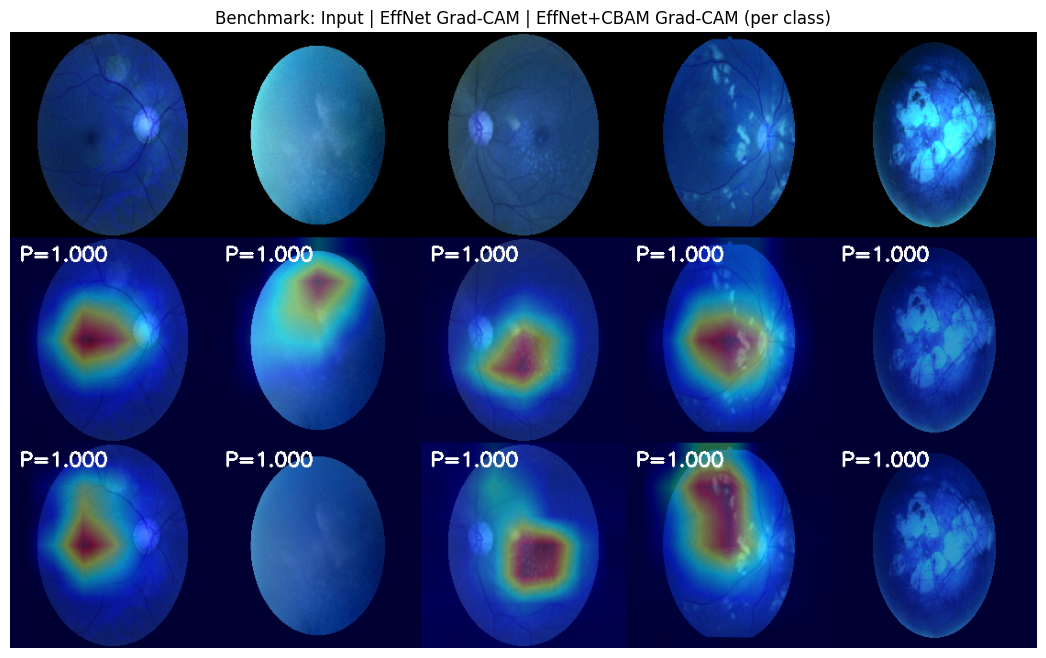
\includegraphics[width=0.98\textwidth]{../new_work/figures/gradcam_benchmark_panel.png}
  \caption{Per\textendash class benchmarking panel: for each class (left to right: Glaucoma, Cataract, AMD, Hypertension, Myopia), we show Input, EffNet Grad\textendash CAM, and EffNet+CBAM Grad\textendash CAM, with class probabilities.}
  \label{fig:gradcam_panel}
\end{figure}

\paragraph{Findings (Benchmark Panel).}
CBAM heatmaps concentrate more tightly on disease\textendash specific anatomy than the baseline across all classes. For Glaucoma, attention centers on the optic disc and neuroretinal rim with less spillover into peripapillary background. For Cataract, CBAM suppresses peripheral artefacts and emphasizes central regions where blur degrades contrast, aligning with global haze signatures rather than spurious vessel noise. For AMD, CBAM highlights macular loci likely corresponding to drusen/RPE changes; even when AMD F1 slightly drops, the spatial focus remains clinically plausible. For Hypertension, CBAM prioritizes arteriole\textendash venule crossings and hemorrhagic spots, consistent with improved recall and PR curves. For Myopia, CBAM attends to posterior pole contours and atrophic patches, although some overlap with macular features explains M\textendash to\textendash A confusions. Compared to the baseline’s broader, sometimes diffuse heatmaps, CBAM produces compact, high\textendash energy regions over relevant structures, which likely reduces overfitting to background textures. The probability annotations show increases for correct classes under CBAM in many examples, indicating alignment between attention focus and classifier confidence. Overall, the panel supports that CBAM’s sequential channel\textendash spatial reweighting yields more clinically meaningful evidence maps.

\begin{figure}[t]
  \centering
  \setlength{\tabcolsep}{6pt}
  \begin{tabular}{ccccc}
    \textbf{G (Glaucoma)} & \textbf{C (Cataract)} & \textbf{A (AMD)} & \textbf{H (Hypertension)} & \textbf{M (Myopia)}\\
    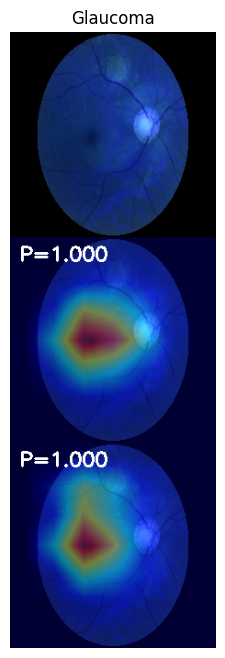
\includegraphics[width=0.18\textwidth]{../new_work/figures/gradcam_benchmark_Glaucoma.png} &
    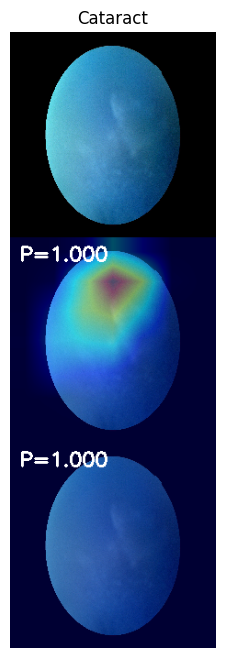
\includegraphics[width=0.18\textwidth]{../new_work/figures/gradcam_benchmark_Cataract.png} &
    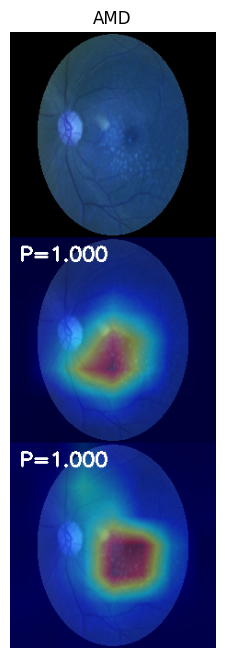
\includegraphics[width=0.18\textwidth]{../new_work/figures/gradcam_benchmark_AMD.png} &
    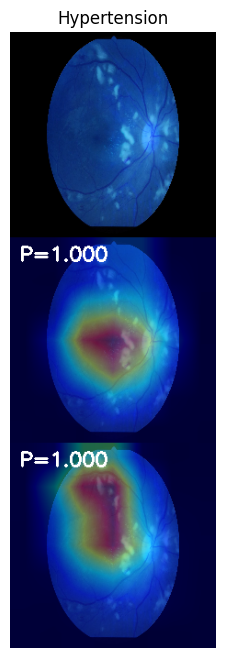
\includegraphics[width=0.18\textwidth]{../new_work/figures/gradcam_benchmark_Hypertension.png} &
    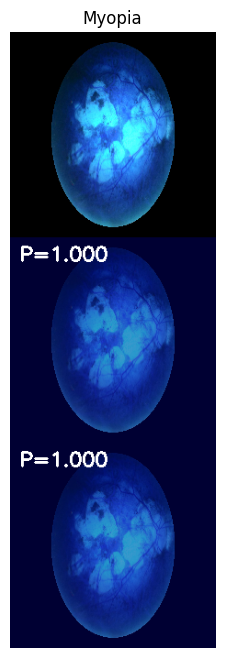
\includegraphics[width=0.18\textwidth]{../new_work/figures/gradcam_benchmark_Myopia.png} \\
  \end{tabular}
  \caption{Per\textendash class examples with explicit class names. Each column shows, from top to bottom: Input, EffNet Grad\textendash CAM (with P), and EffNet+CBAM Grad\textendash CAM (with P).}
  \label{fig:gradcam_perclass}
\end{figure}

\paragraph{Findings (Per\textendash Class Grad\textendash CAM).}
For G, CBAM reduces activation over vessels distant from the disc and concentrates on cup\textendash to\textendash disc geometry, matching clinical salience. For C, CBAM highlights central blur patterns and de\textendash emphasizes sharp peripheral textures, reinforcing that it learns global degradation cues. For A, CBAM focuses on parafoveal macular regions; when errors occur, heatmaps still target plausible drusen areas, indicating threshold/imbalance rather than focus drift. For H, CBAM’s high\textendash intensity patches track AV crossings, arteriolar narrowing, and blot hemorrhages, which explains the large recall jump. For M, CBAM outlines the posterior pole and atrophic patches consistent with staphyloma; overlap with macular anomalies clarifies occasional M\textendash to\textendash A confusions. Across classes, CBAM’s spatial masks are more compact and less noisy than the baseline, and the associated probabilities tend to be higher on correctly focused regions. These case studies corroborate quantitative patterns: attention sharpens evidence on relevant structures, reduces spurious background reliance, and improves minority class behavior without adding heavy computational cost.

\paragraph{Discussion.} Consistent with prior analyses of CBAM \cite{cbamDO,cbamMedium,woo2018cbam}, our overlays show that CBAM suppresses background and sharpens disease\textendash specific structures. For AMD and Myopia, CBAM concentrates on macular and optic\textendash disc vicinity more consistently than the baseline. Hypertension remains challenging due to scarce single\textendash label samples; however, row\textendash normalized confusion indicates improved precision compared to recall, suggesting additional class weighting and data curation can further benefit H.

